\documentclass{beamer}

\usepackage[utf8]{inputenc}
\usepackage{amsfonts}
\usepackage{amsmath}
\usepackage{xcolor}
\usepackage[noend]{algpseudocode}
\usefonttheme{serif}
\usetheme{Boadilla}
\usecolortheme{seahorse}

\title[Foraging]{Biomimicry of Bacterial Foraging}
\subtitle{for Distributed Optimization and Control}
\author[Passino; Van de Kleut]{
  Kevin M. Passino\inst{1}\\
  Presented by: Alexander Van de Kleut\inst{2}
}
\institute[OST; UW]{\inst{1}
  The Ohio State University\\
  Electrical and Computer Engineering
  \and
  \inst{2}
  University of Waterloo\\
  Centre for Theoretical Neuroscience
}
\date[W20]{IEEE Control Systems Magazine, 2002}

\begin{document}

% Today I'm going to be presenting the paper "Biomimicry of Bacterial Foraging for Distributed Optimization and Control" by Kevin Passino.
% Kevin Passino is a professor at the Ohio State University working in Electrical and Computer Engineering. Passino has done a lot of work in many fields, but some of his most influential work has been in the field of biologically-inspired metaheuristics for optimization.
% This paper is his most-cited work in this field with over 3000 citations. In this paper, Passino develops a model of how colonies of the bacteria E. coli forage for food, and implements this model as an optimization algorithm.
\frame{\titlepage}

% There are going to be three main sections to my presentation.
% The first is discussing the background on E. coli, foraging, and how foraging might be used as an optimization algorithm.
% The second section, which makes up the bulk of the presentation, is a step-by-step guide on how the final algorithm might be built up. We have discussed in class how crucial reproducability is for papers, especially papers in computer science and biology. Despite the fact that every paper we have read is essentially presenting an algorithm, not many papers take the time to clearly explain the algorithm. This paper is longer than the others and includes an entire page dedicated to the algorithm itself. This actually enabled me to write the algorithm myself with basically no issues in just a few hours. My goal today is for you guys to come away being able to implement this algorithm yourself as well.
% The third and final section will be a discussion of the algorithm and the paper itself, with a few critiques. I will then open the floor for discussion.
% I also have some extra results at the end so if you want to see them, make sure to ask during the question phase!
\begin{frame}
\frametitle{Outline}
\tableofcontents
\end{frame}

\section{Foraging as Optimization}


% So let's define this crucial term: foraging. What is foraging?
% At it's most basic, foraging just means searching for food or nutrients in the environment. It also means simultaneously avoiding dangers, like toxins or predators, which biologists call "noxious stimuli".
% Social foraging is a kind of foraging that happens "as a group".
% Social foraging is good because it can increase the likelihood of finding nutrients by covering more ground, and it can decrease the likelihood of encountering noxious stimuli and provide protection. this is a good strategy when the gains from social foraging offset the costs of competition for food.
\begin{frame}
\frametitle{Foraging}
\begin{itemize}
  \item<1-> \textbf{Foraging}
  \begin{itemize}
    \item<1-> searching for nutrients
    \item<1-> avoiding noxious stimuli (toxins, predators, etc)
  \end{itemize}
  \item<2-> \textbf{Social Foraging}
  \begin{itemize}
    \item<2-> increases likelihood of finding nutrients
    \item<2-> better detection and protection from noxious stimuli
    \item<2-> gains can offset cost of food competition
  \end{itemize}
\end{itemize}
\end{frame}

% Passino's key insight while learning about foraging behaviours in nature was that foraging is a kind of optimization algorithm.
% We can think of foraging as trying to minimize some loss function $J$ acting on some parameters $\theta$. In this case, $\theta$ represents the position of an animal, and $J$ represents how good that position is. For example J can be lower where there are more nutrients and higher where there are more noxious stimuli. By minimizing J, the animal avoids dangers and finds food sources - foraging.
% But of course, as computer scientists do, if we abstract away the ecological meanings of $J$ and $\theta$, we see that foraging is a kind of optimization process.
\begin{frame}
\frametitle{Foraging as Optimization}
\textbf{How can we view foraging as an Optimization Process?}
\begin{itemize}
  \item<1-> We have some parameters $\theta$ and a loss function $J(\theta)$ that we want to minimize
  \item<2-> $\theta$ can represent the position of an organism in its environment
  \item<3-> $J$ can represent the concentration of nutrients and noxious stimuli
  \begin{itemize}
    \item smaller values of $J$ = more nutrients, less noxious stimuli
    \item higher values of $J$ = more noxious stimuli, less nutrients
  \end{itemize}
  \item<4-> In general, $J$ and $\theta$ can be arbitrary
  \begin{itemize}
    \item $\theta \in \mathbb{R}^p$
    \item $J: \mathbb{R}^p \to \mathbb{R}$
  \end{itemize}
\end{itemize}
\end{frame}

% Passino wanted to model his foraging algorithm after a particular organism. The goal was not just to develop a new optimization algorithm, but to also try to model the foraging behaviour of an existing organism.
% He landed on E. coli as his organism of choice.
% E. coli is a model organism: probably the most studied organism. We have characterized its foraging behaviour through ecological studies so we have a good basis for our algorithm. Also, its a relatively simple organism so we probably won't feel too bad about simplifying its behaviour for modelling.
% It's also a social organism, so it engages in social foraging. It secretes chemical signals into the environment that attract nearby E. coli, resulting in swarms of clumps of bacteria.
\section{Building the Algorithm}
\begin{frame}
\frametitle{\textit{E. coli}}
\begin{itemize}
  \item<1-> Model organism
  \begin{itemize}
    \item<1-> Highly studied
    \item<1-> Well-characterized foraging behaviour
    \item<2-> Probably won't feel bad about simplifying its behaviour
  \end{itemize}
  \item<3-> Social organism
  \begin{itemize}
    \item<3-> Secretes signals to attract others nearby
    \item<3-> Encourages ``swarming'' or ``clumping''
  \end{itemize}
\end{itemize}
\end{frame}

% E. coli move around by swimming. Their bodies are covered in helical proteins called 'flagella' that act like tiny properllows.
% The flagella let the E. coli move in two ways. If all the flagella rotate clockwise, then they all pull outwards, causing the cell to move randomly. We call this tumbling.
% If they all rotate counterclockwise, then they all tend to wrap together and form one big propeller which moves it in a single direction. We call this running.
\begin{frame}
\frametitle{\textit{\textit{E. coli}} Behaviour}
\begin{itemize}
  \item<1-> Swims using left-handed helical flagella (``propellers'')
  \begin{itemize}
    \item<2-> \textbf{Tumble}: flagella all rotate clockwise $\to$ pull on cell in all directions $\to$ random movement
    \item<3-> \textbf{Run}: flagella all rotate counterclockwise $\to$ flagella form a bundle $\to$ push on cell in one direction $\to$ directed movement
  \end{itemize}
\end{itemize}
\begin{center}
\includegraphics<1->[scale=0.2]{assets/ecoli}
\end{center}
\end{frame}

% So when does it tumble, and when does it run?
% If E. coli happens to swim *down* a nutrient concentration gradient (meaning it goes from less to more concentrated nutrients) then it tends to prolong how long it spends running.
% Otherwise, it tends to switch into a tumble to randomly search for a better direction for movement.
% We call tumbling followed by potentially running a 'chemotaxis step'.
\begin{frame}
\frametitle{\textit{\textit{E. coli}} Behaviour}
\begin{itemize}
  \item<1-> If during a tumble \textit{\textit{E. coli}} swims down a nutrient concentration gradient:
  \begin{itemize}
    \item<1-> Prolongs time spent on a run
    \item<1-> Continues moving in the same direction
  \end{itemize}
  \item<2-> Otherwise:
  \begin{itemize}
    \item<2-> Tends to switch to a tumble (search for more)
    \item<2-> Moves randomly which searching for more nutrient gradients to exploit
  \end{itemize}
  \item<3-> Call a tumble followed by a run a ``chemotaxis step''
\end{itemize}
\end{frame}

% So let's encode this idea of a chemotaxis step into an algorithm.
% Let's say we want to let a bacterium forage for $N_c$ time steps
% first, we pick a random direction to move in. Let's call that $\phi$. The notation here means "$\phi$ is a random unit vector in p dimensions"
% then, we move in the direction given by $\phi$ by some step size $c$ which tells us how far we can move per time step.
% then, if continuing to move in that direction causes a decrease in the objective function, continue to move in that direction.
\begin{frame}
\frametitle{Algorithm for a Single Bacterium}
\begin{algorithmic}[1]
\For {$j \gets 1 \dots N_c $}:
  \State $\phi \sim S^p$
  \State $\theta \gets \theta + c \phi$
  \While {$J(\theta + c \phi) < J(\theta)$}:
    \State $\theta \gets \theta + c \phi$
  \EndWhile
\EndFor
\end{algorithmic}
\begin{itemize}
  \item $\theta$: $p$-dimensional vector (randomly initialized)
  \item $N_c$: number of chemotaxis steps
  \item $\phi \sim S^p$: a random $p$-dimensional unit vector
  \item $c$: a step-size
\end{itemize}
\end{frame}

% So let's try this algorithm out. This is an image of a classical loss function in nonconvex optimization. This is the 'rastrigin function'. It has local minima at integer coordinates and a global minimum at 0.
% This is a challenging function to minimize because most gradient-based optimizers tend to get stuck at local optima.
\begin{frame}
\frametitle{Loss Function to Optimize}
\begin{center}
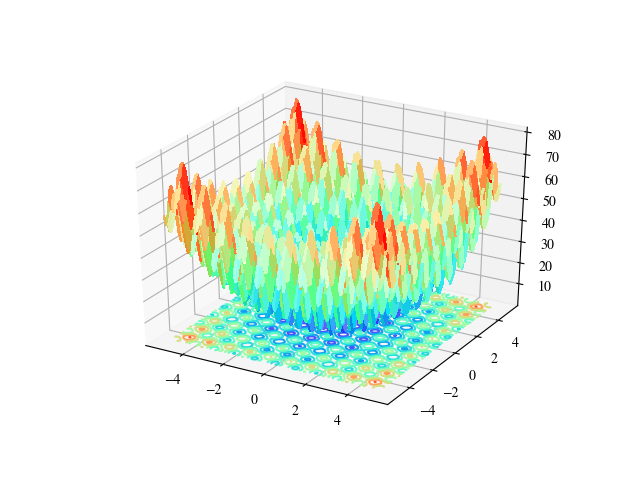
\includegraphics[scale=0.5]{assets/rastrigin}
$$J(\theta) = An + \sum_{i=1}^n \left( x_i^2 - A \cos(2 \pi x_i) \right)$$
\end{center}
\end{frame}

% So if we run this algorithm a number of times, these are the results.
% The first image shows the value of $J$ over iterations, with a different plot for each independent run. The number $J^*$ in the middle is the minimum value found during the optimization process.
% The second plot shows the paths taken by each bacterium on their run, plotted over top of a contour plot of the rastrigin function.
% We can see that the performance is inconsistent and so running the algorithm just once is unreliable.
\begin{frame}
\frametitle{Results of Single Bacterium}
\begin{columns}[T]
  \column{0.5\textwidth}
    \begin{center}
      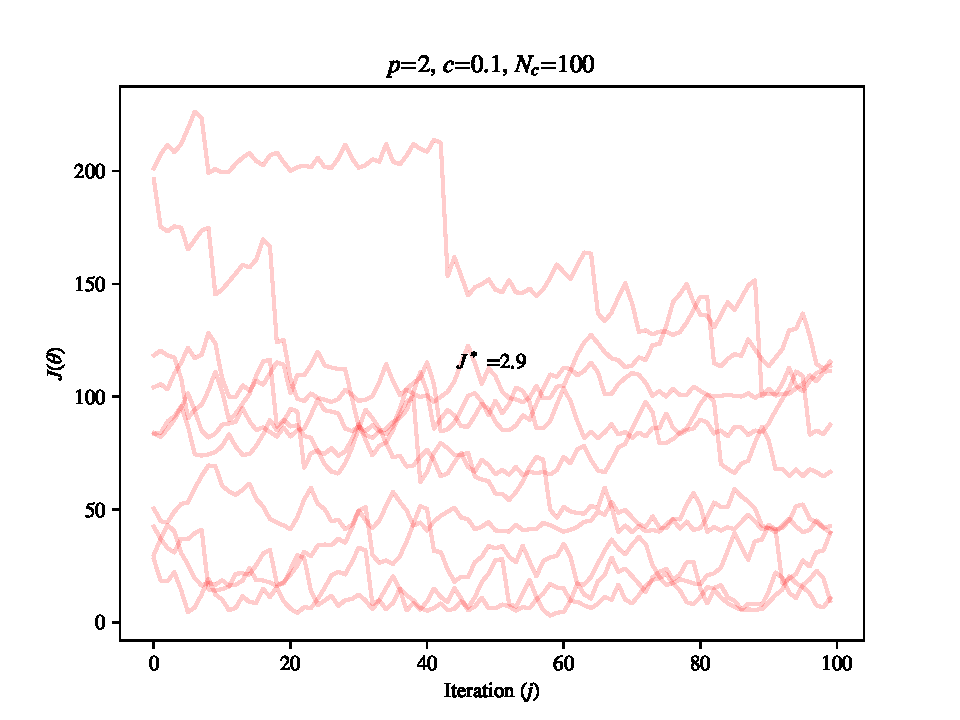
\includegraphics[scale=0.3]{assets/rastrigin_J}
      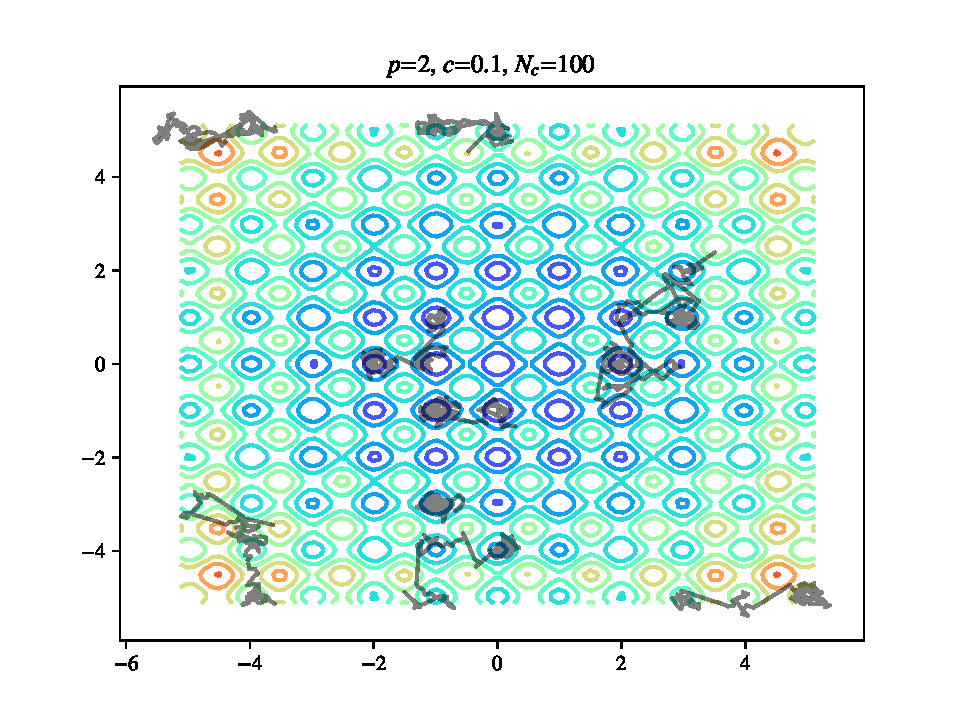
\includegraphics[scale=0.3]{assets/rastrigin_theta}
    \end{center}
  \column{0.5\textwidth}
    \begin{itemize}
      \item Highly variable performance between different initializations
      \item This algorithm alone is too unreliable to get good performance
    \end{itemize}
\end{columns}
\end{frame}

% We might think "oh just run it multiple times!"
% But Passino had a better idea. He knew that E. coli did social foraging. They secrete chemicals into the environment that attract other nearby bacteria
% They can't attract nearby bacteria arbitrarily close, so once bacteria are close enough, they repel each other.
% Passino used two gaussian functions to model this.
\begin{frame}
\frametitle{$J_{cc}$ and swarming behaviour}
\begin{itemize}
  \item \textit{\textit{E. coli}} do social foraging
  \item Secrete a substance to indicate to attract nearby \textit{\textit{E. coli}} and encourage swarming
  \item Strength of signal diffuses over space
  \item Also want to avoid crowding
  \item Use sum of two Gaussian functions to model this
\end{itemize}
\end{frame}

% One gaussian is negative and corresponds to the attraction between cells. It has two parameters, d_attract and w_attract controlling the depth and width of the attraction.
% The second is positve and corresponds to the repulsion between cells. It has the same parameters.
% By adding them together, we get this auxiliary function $J_cc$, where cc means cell-to-cell. By adding $J_cc$ to the original function we are minimizing, we can add swarming behaviour to the optimization process.
\begin{frame}
\frametitle{$J_{cc}$ and swarming behaviour}
\begin{center}
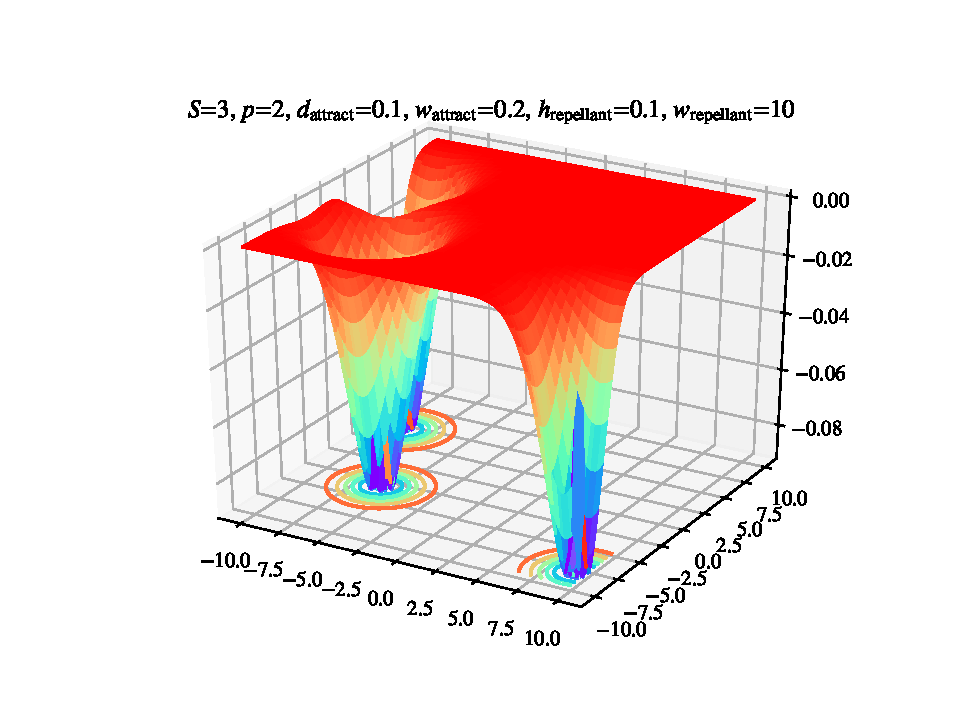
\includegraphics[scale=0.4]{assets/swarming}
\begin{align*}
J_{cc}(\theta) = \sum_{i=1}^S &-d_\text{attract} \exp \left( -w_\text{attract} (\theta - \theta_i)^T (\theta - \theta_i) \right) \\ &+ h_\text{repellant} \exp \left( -w_\text{repellant} (\theta - \theta_i)^T (\theta - \theta_i) \right)
\end{align*}
\end{center}
\end{frame}

% So to add this in to our algorithm, we are going to need not one bacterium, but many. We use $S$ for swarm to indicate the number of bacterium.
% Our new algorithm is almost identical to the original.
% the outer for loop over the chemotaxis steps is the same
% but now we have an extra for loop over the bacterium in the colony
% we have a value of theta for each bacterium called $\theta_i$ as well as a step size for each bacterium called $c_i$.
% we also add $J_cc$ to the loss function to encourage swarming.
\begin{frame}
\frametitle{Algorithm for a Colony}
\begin{algorithmic}[1]
\For {\textcolor{gray}{$j \gets 1 \dots N_c $}}:
  \For {$i \gets 1 \dots S$}:
    \State \textcolor{gray}{$\phi \sim S^p$}
    \State \textcolor{gray}{$\theta_i \gets \theta_i + c_i \phi$}
    \While {\textcolor{gray}{$J(\theta_i + c_i \phi)$} $+ J_{cc}(\theta_i + c_i \phi)$ \textcolor{gray}{$< J(\theta_i) $} $+ J_{cc}(\theta_i)$}:
      \State \textcolor{gray}{$\theta_i \gets \theta_i + c_i \phi$}
    \EndWhile
  \EndFor
\EndFor
\end{algorithmic}
\begin{itemize}
  \item $\theta_i$: $i$th $p$-dimensional vector (randomly initialized)
  \item $S$: number of bacteria in the colony
  \item $c_i$: a step-size for bacterium $i$
  \item $J_cc$: cell-to-cell interactions
\end{itemize}
\end{frame}

% Here are the results of adding in swarming. This time the plot shows the losses of each bacterium in the colony for a single colony. It doesn't really look much better than before, so is this really a good addition?
% Well remember, we added four new hyperparameters that we have to tune. So let's see if we can get better performance by changing the hyperparameters.
\begin{frame}
\frametitle{Results of Colony with Swarming}
\begin{columns}[T]
  \column{0.5\textwidth}
    \begin{center}
      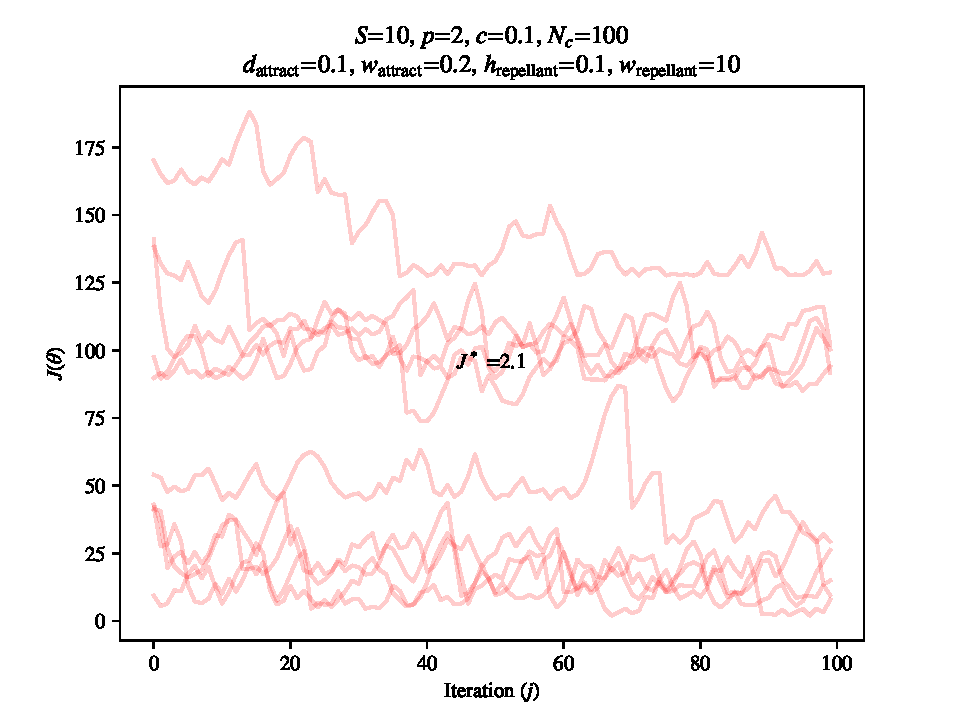
\includegraphics[scale=0.3]{assets/rastrigin_colony_J}
      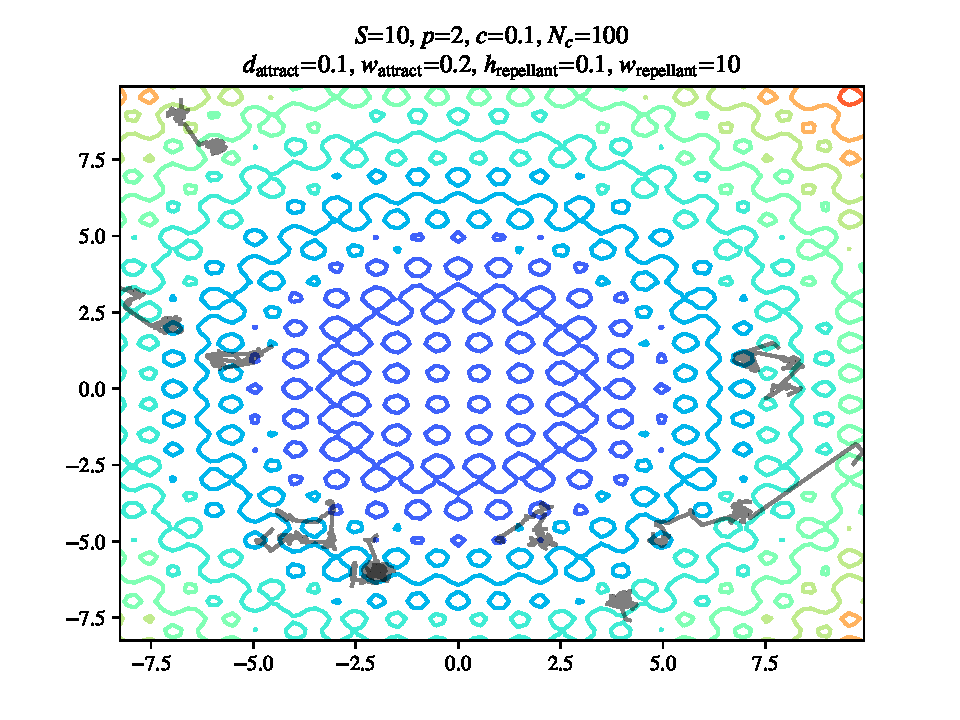
\includegraphics[scale=0.3]{assets/rastrigin_colony_theta}
    \end{center}
  \column{0.5\textwidth}
    \begin{itemize}
      \item Still relatively inconsistent performance for a highly nonconvex function
      \item But wait... What if the problem is just the hyperparameters?
    \end{itemize}
\end{columns}
\end{frame}

% To get these hyperparameters I just picked a few random combinations and tested them. This improved the overall performance. I increased the values of all of the hyperparameters, especially the ones for attraction. The $J_cc$ function output values on a much smaller scale than $J$ so it wasn't influential enough originally.
% It's important to know the scales of these two functions since it gives a tradeoff between local and global behaviour for each bacterium, kind of like the hyperparameters for PSO.
\begin{frame}
\frametitle{Results of Colony with Swarming}
\begin{columns}[T]
  \column{0.5\textwidth}
    \begin{center}
      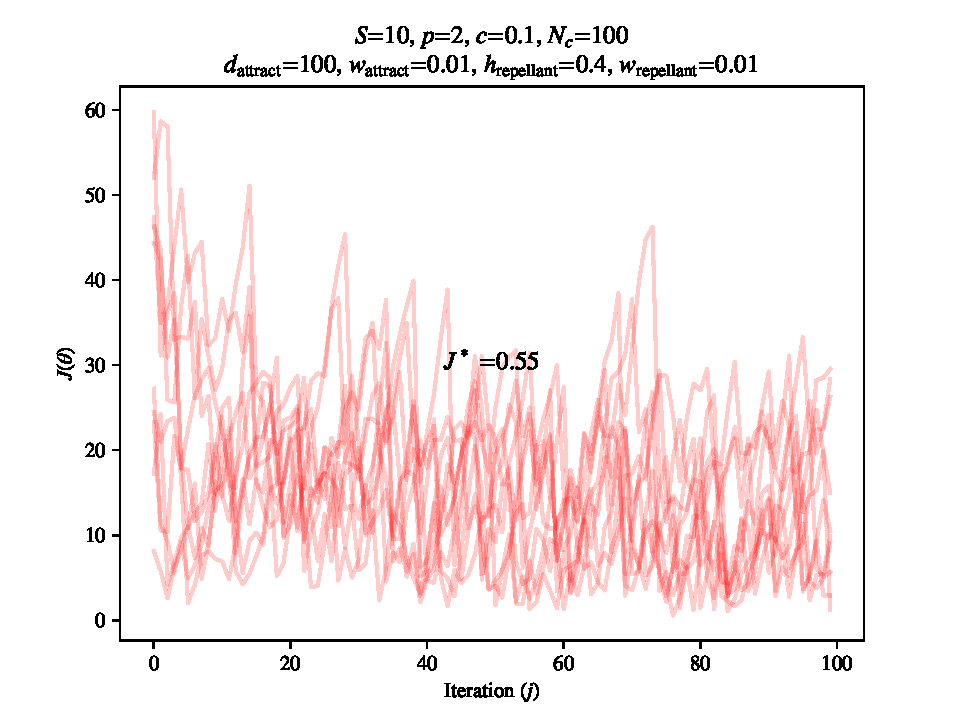
\includegraphics[scale=0.3]{assets/rastrigin_colony_tuned_J}
      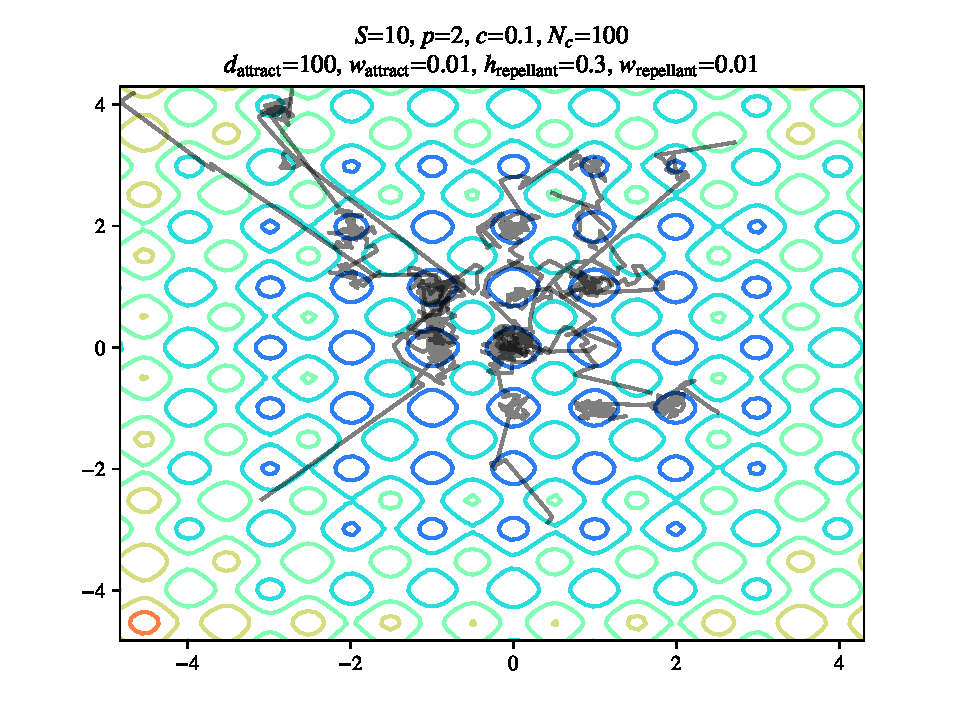
\includegraphics[scale=0.3]{assets/rastrigin_colony_tuned_theta}
    \end{center}
  \column{0.5\textwidth}
    \begin{itemize}
      \item<1-> By trying out different combinations of hyperparameters we can improve overall performance
      \item<1-> Here we increased the depth and width of attraction as well as the depth and width of repellance to increase "global" behaviour
      \item<2-> Important to know scale of $J$ relative to scale of $J_{cc}$ for tradeoff
      \begin{itemize}
        \item<2-> Can think of this like hyperparameters $c_1$ and $c_2$ for PSO
      \end{itemize}
    \end{itemize}
\end{columns}
\end{frame}

% This is just an image showing the before hyperparameters, which are taken from the paper, and the after, which were found by random sampling.
\begin{frame}
\frametitle{Comparing $J_{cc}$}
\begin{columns}[T]
  \column{0.5\textwidth}
  \begin{center}
    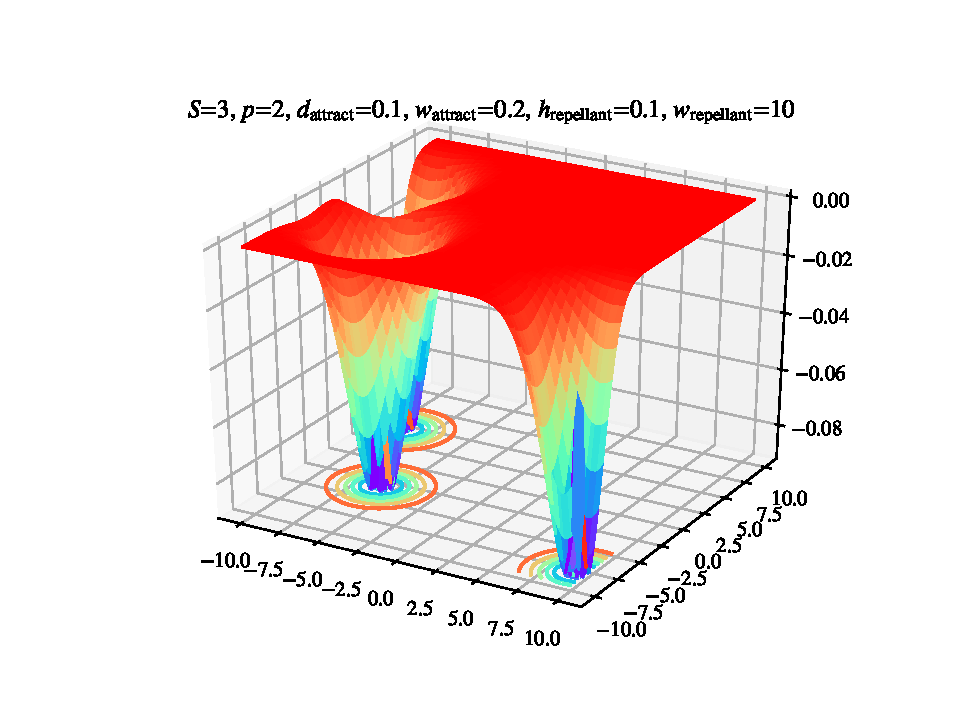
\includegraphics[scale=0.4]{assets/swarming}
  \end{center}
  \column{0.5\textwidth}
  \begin{center}
    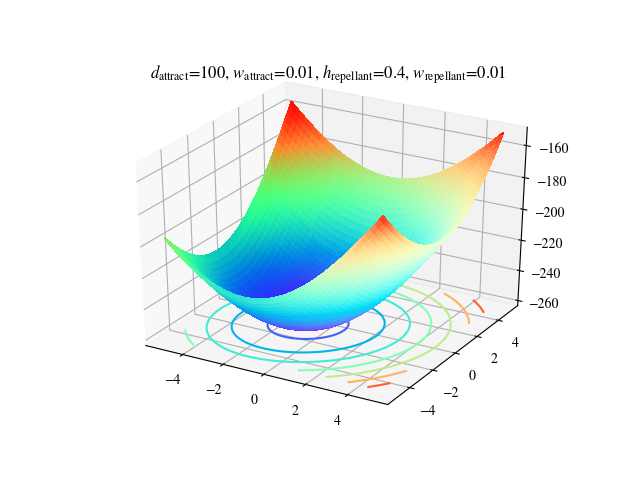
\includegraphics[scale=0.4]{assets/swarming_tuned}
  \end{center}
\end{columns}
\end{frame}

% Can we make this algorithm better and more biologically inspired?
% Let's introduce reproduction into the picture. In nature, E. coli reproduce in two ways: binary fission and horizontal translation. In binary fission, the E. coli is basically copy and pasted.
% Passino added binary fission to his model of E. coli foraging by taking the weakest half of the population and killing them off, and duplicating the strongest half of the population. He defines weakest and strongest in terms of the total value of the loss function experienced over the last iteration.
\begin{frame}
\frametitle{\textit{E. coli} reproduction}
\begin{itemize}
  \item<1-> \textit{E. coli} ``reproduce'' via binary fission, which essentially produces a clone
  \item<2-> Individuals with higher values of $J$ killed off
  \item<3-> Individuals with lower values of $J$ duplicated
  \begin{itemize}
    \item<3-> Ideally move away due to repellance
  \end{itemize}
  \item<4-> Idea is to encourage searching in space nearby ``best'' individuals
  \item<5-> \alert{If repellance isn't high enough then repeated iterations of evolution can concentrate colony in local minimum}
\end{itemize}
\end{frame}

% To add this to our algorithm is pretty simple: Just add an outer for loop that loops over generations. After the inner optimization loops are done, just take the best half and clone them, and delete the worst half.
\begin{frame}
\frametitle{Algorithm for a Reproducing Colony}
\begin{algorithmic}[1]
\For {$k \gets 1 \dots N_{re}$}:
  \For {\textcolor{gray}{$j \gets 1 \dots N_c $}}:
    \For {\textcolor{gray}{$i \gets 1 \dots S$}}:
      \State \textcolor{gray}{$\phi \sim S^p$}
      \State \textcolor{gray}{$\theta_i \gets \theta_i + c_i \phi$}
      \While {\textcolor{gray}{$J(\theta_i + c_i \phi) + J_{cc}(\theta_i + c_i \phi) < J(\theta_i) + J_{cc}(\theta_i)$}}:
        \State \textcolor{gray}{$\theta_i \gets \theta_i + c_i \phi$}
      \EndWhile
    \EndFor
  \EndFor
  \State delete worst $S/2$ and reproduce best $S/2$
\EndFor
\end{algorithmic}
\begin{itemize}
  \item $N_{re}$: number of reproduction steps
\end{itemize}
\end{frame}

% Let's see the results. Here I've run the algorithm with 4 generations, coloured red, green, blue, and cyan.
% It looks like adding reproduction can help a bit by concentrating the population in more promising areas. Like we said, this can be a good or bad thing. It also adds another tuning parameter - how do we know when to stop reproducing?
\begin{frame}
\frametitle{Results of Reproducing Colony}
\begin{columns}[T]
  \column{0.5\textwidth}
    \begin{center}
      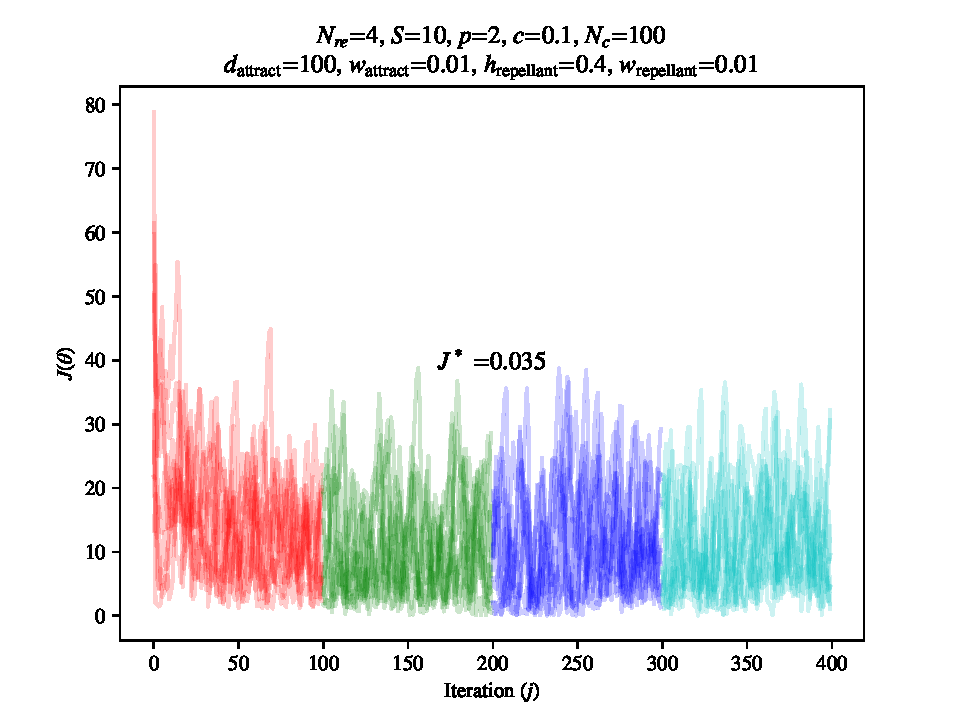
\includegraphics[scale=0.3]{assets/rastrigin_colony_re_J}
      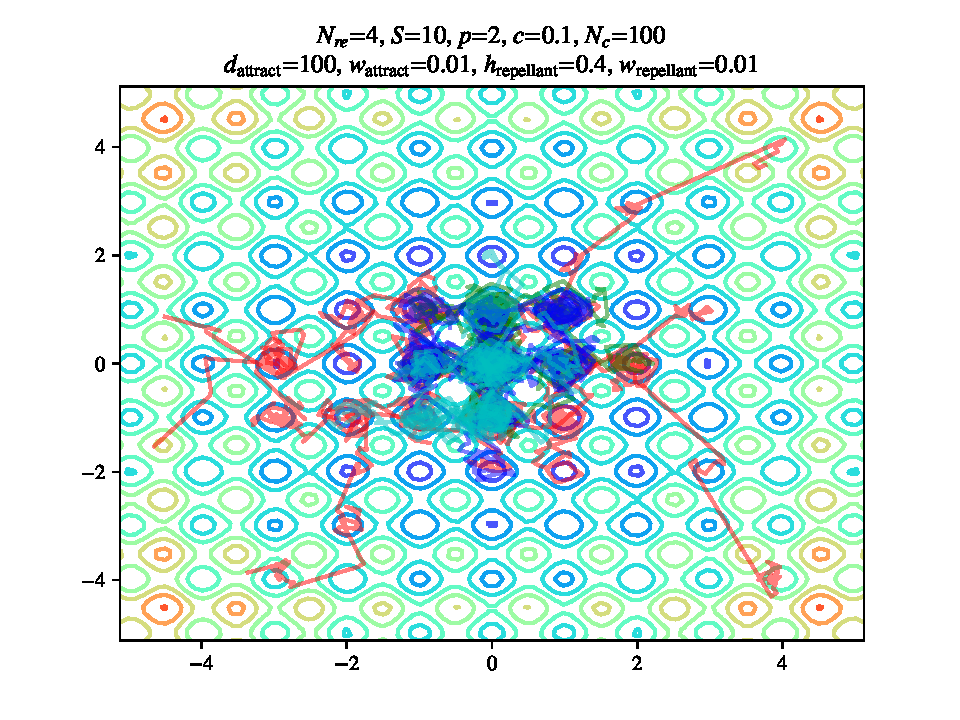
\includegraphics[scale=0.3]{assets/rastrigin_colony_re_theta}
    \end{center}
  \column{0.5\textwidth}
  \begin{itemize}
    \item<1-> Adding reproduction improves performance
    \item<2-> Concentrates population in more promising areas of the search space
    \item<3-> Adds another tuning parameter - how do we know how many generations is enough?
  \end{itemize}
\end{columns}
\end{frame}

% You might be wondering if reproduction actually helps. By adding an outer for loop we basically increase how long we are optimizing for. So what if we just ran the algorithm without reproduction for the same number of iterations?
% We get pretty similar results, but it's possible that reproduction does provide an edge over just iterating longer.
\begin{frame}
\frametitle{Does Reproduction Help?}
\begin{columns}[T]
  \column{0.5\textwidth}
    \begin{center}
      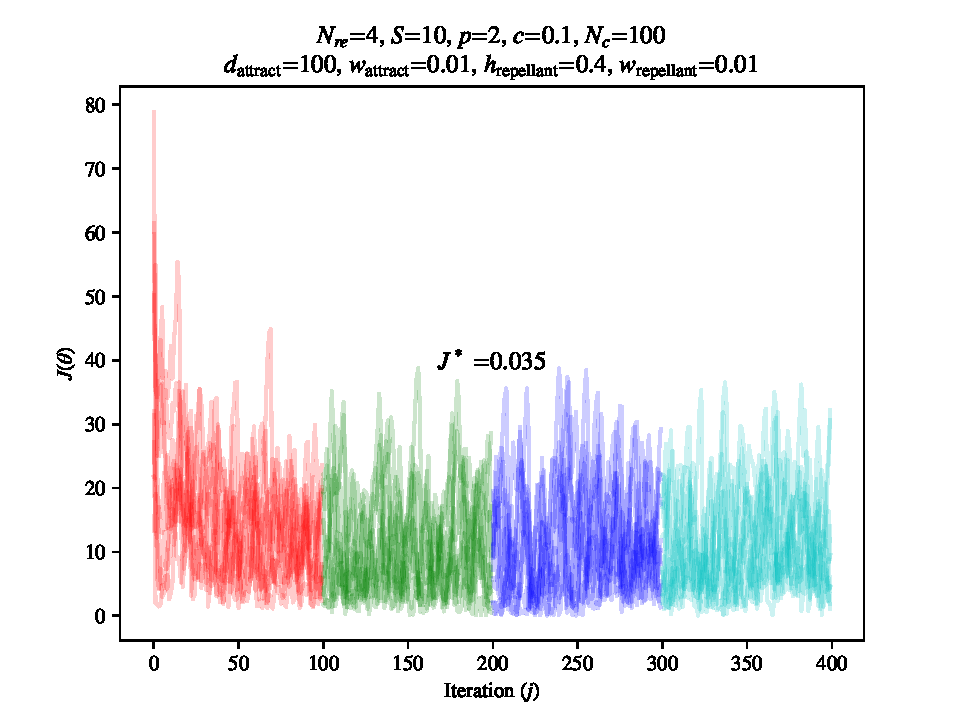
\includegraphics[scale=0.3]{assets/rastrigin_colony_re_J}
      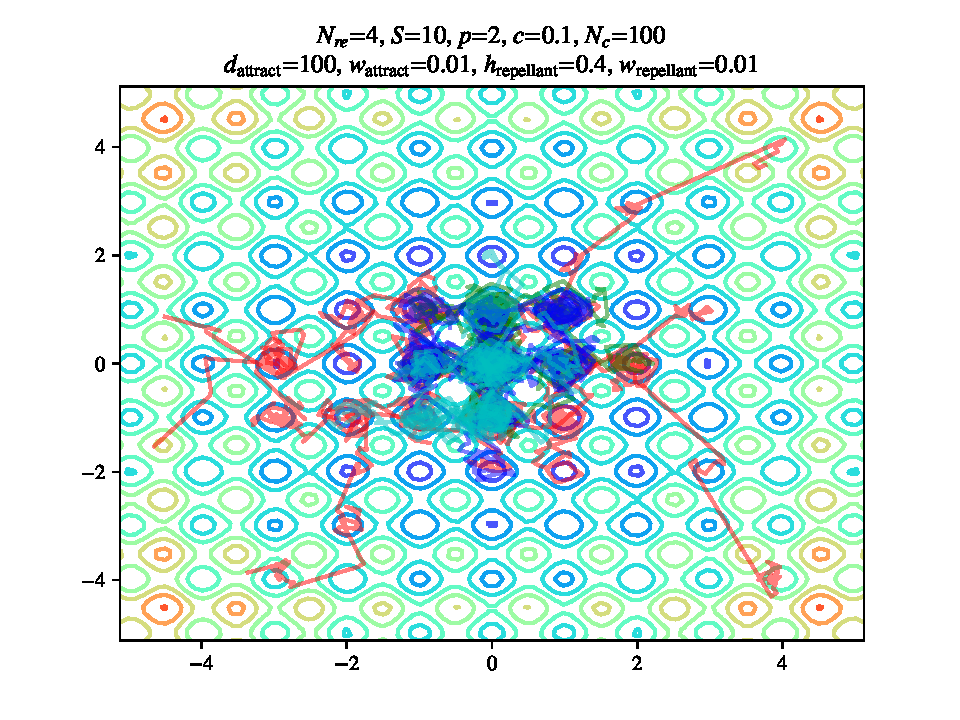
\includegraphics[scale=0.3]{assets/rastrigin_colony_re_theta}
    \end{center}
  \column{0.5\textwidth}
  \begin{center}
    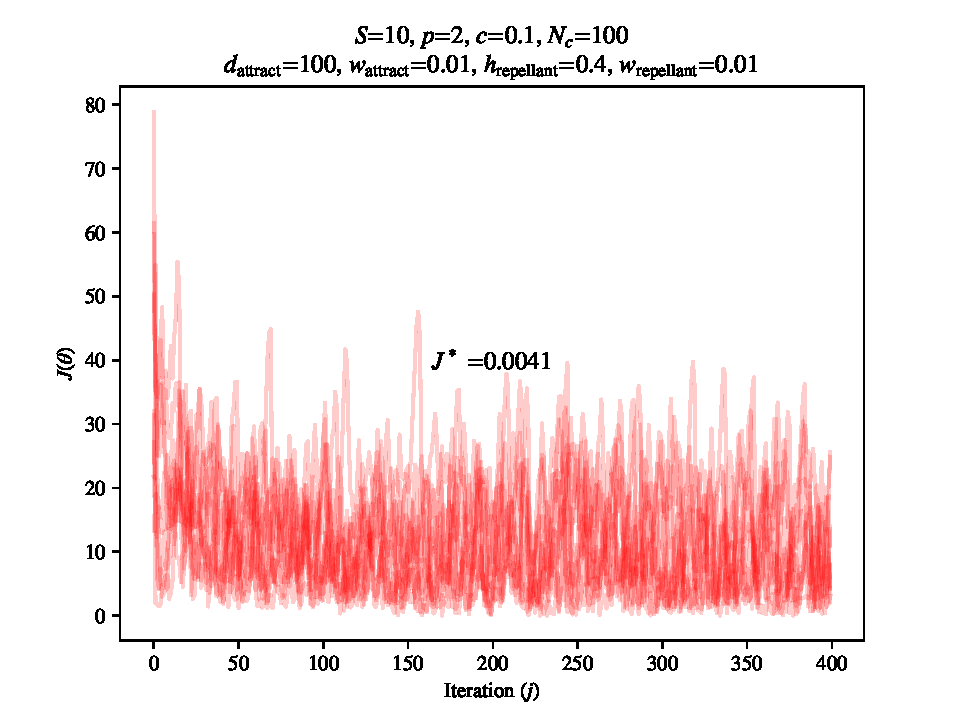
\includegraphics[scale=0.3]{assets/rastrigin_colony_400_J}
    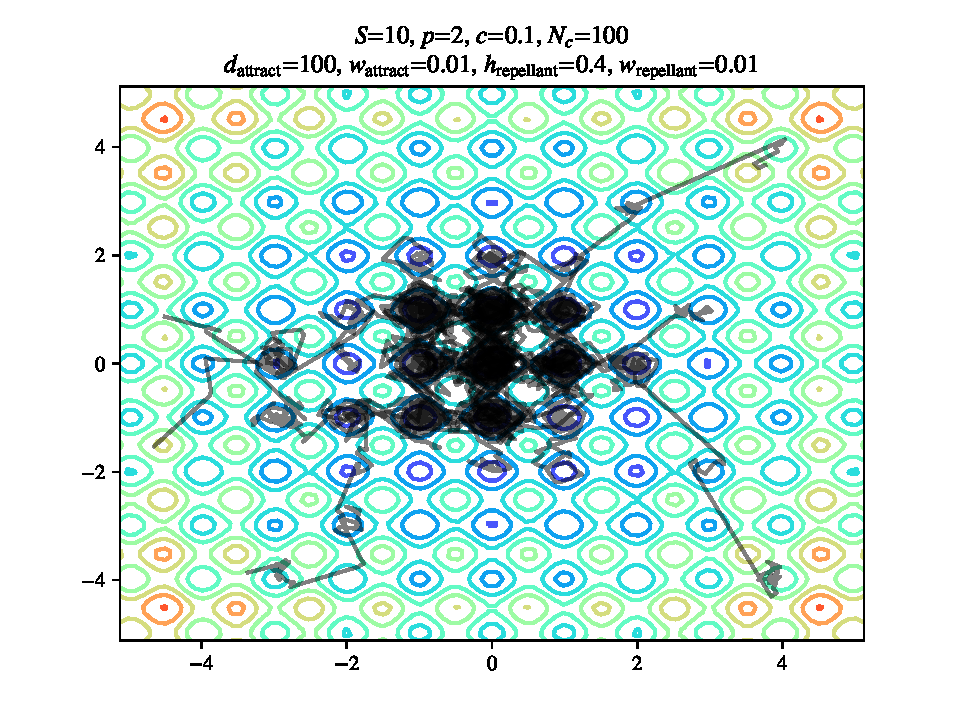
\includegraphics[scale=0.3]{assets/rastrigin_colony_400_theta}
  \end{center}
\end{columns}
\end{frame}

% The last piece of the puzzle that Passino wanted to include in his model of E. coli foraging is elimination-dispersal events.
% These are basically random events that disperse bacteria from one place to another. For example, through waterways, from animal activity or from things humans are doing like coughing then shaking hands.
% While this may destroy some chemotactic progress, it can also transport E. coli to places it might never have reached alone.
% In terms of optimization, this can help prevent getting stuck in a local minimum.
\begin{frame}
\frametitle{Elimination-Dispersal Events}
\begin{columns}[T]
\column{0.5\textwidth}
\begin{center}
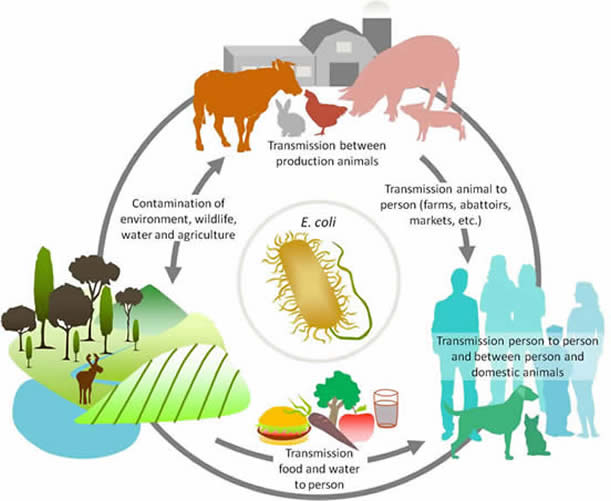
\includegraphics[scale=0.25]{assets/transmission.jpg}
\end{center}
\column{0.5\textwidth}
\begin{itemize}
  \item<1-> Over time, random events disperse populations of \textit{E. coli}
  \begin{itemize}
    \item<1-> Water, animal activity, human intervention
  \end{itemize}
  \item<2-> May destroy chemotactic progress
  \begin{itemize}
    \item<2-> But may also bring \textit{E. coli} to good food sources
  \end{itemize}
  \item<3-> For optimization, this is a method to prevent stagnation and move out from local minima
\end{itemize}
\end{columns}
\end{frame}

% To add this to our algorithm, we add yet another outer for loop for the number of elimination-dispersal events.
% We also add a for loop through the colony that sets $\theta$ to a random vector from the initial distribution of $\theta$ with probabilty $p_ed$. This is the idea that every so often some of the bacteria are randomly displaced and spread out.
\begin{frame}
\frametitle{Algorithm for a Dispersing Colony}
\begin{algorithmic}[1]
\For {$l \gets 1 \dots N_{ed}$}:
  \For {\textcolor{gray}{$k \gets 1 \dots N_{re}$}}:
    \For {\textcolor{gray}{$j \gets 1 \dots N_c $}}:
      \For {\textcolor{gray}{$i \gets 1 \dots S$}}:
        \State \textcolor{gray}{$\phi \sim S^p$}
        \State \textcolor{gray}{$\theta_i \gets \theta_i + c_i \phi$}
        \While {\textcolor{gray}{$J(\theta_i + c_i \phi) + J_{cc}(\theta_i + c_i \phi) < J(\theta_i) + J_{cc}(\theta_i)$}}:
          \State \textcolor{gray}{$\theta_i \gets \theta_i + c_i \phi$}
        \EndWhile
      \EndFor
    \EndFor
    \State \textcolor{gray}{delete worst $S/2$ and reproduce best $S/2$}
  \EndFor
  \For {$i \gets 1 \dots S$}:
    \If {$\epsilon \sim \mathcal{U}(0, 1) < p_{ed}$}:
      \State $\theta_i \sim d^0(\theta)$
    \EndIf
  \EndFor
\EndFor
\end{algorithmic}
\begin{itemize}
  \item $N_{ed}$: number of elimination-dispersal events
  \item $p_{ed}$: probabilty of a single elimination-dispersal event
  \item $d^0(\theta)$: initial distribution of $\theta$
\end{itemize}
\end{frame}

% Here I have four frames showing the inner optimization process following elimination-dispersal events. The overall best value achieved is even lower than before, so elimination-dispersal seems to be helpful. However, we can also see that sometimes the best value achieved over many generations is worse than before, so it doesn't always lead to a monotonic decrease in the loss function.
% Overall, it seems like the algorithm is quite strong, being able to find solutions to the optimization problem that are close to the global minimum.
\begin{frame}
\frametitle{Results of Elimination-Dispersal}
\begin{columns}[T]
  \column{0.5\textwidth}
    \begin{center}
      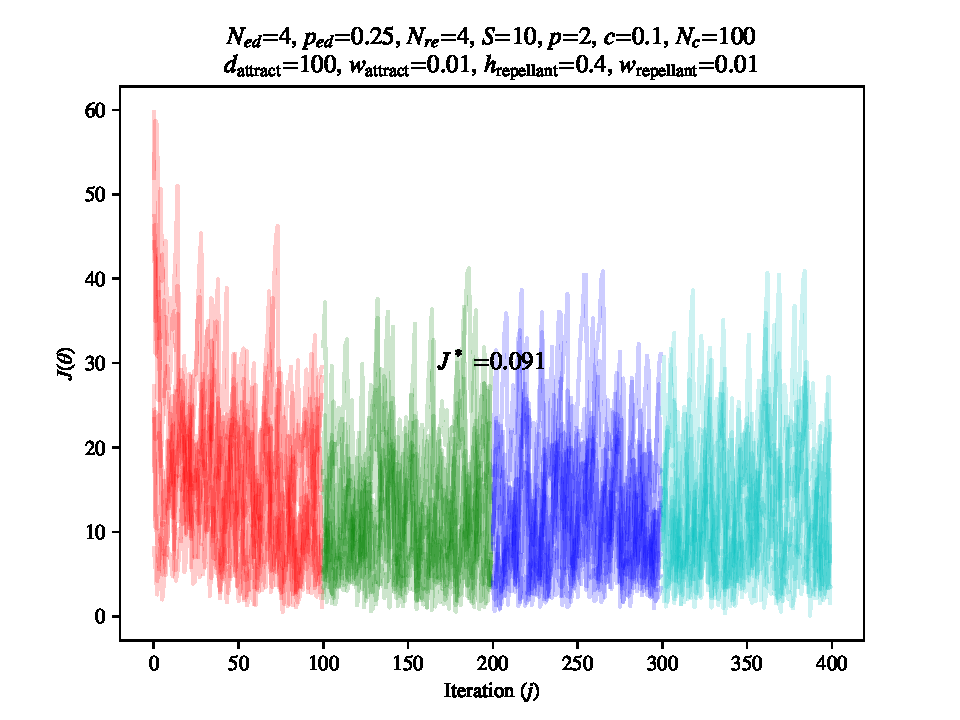
\includegraphics[scale=0.3]{assets/rastrigin_colony_ed_0_J}
      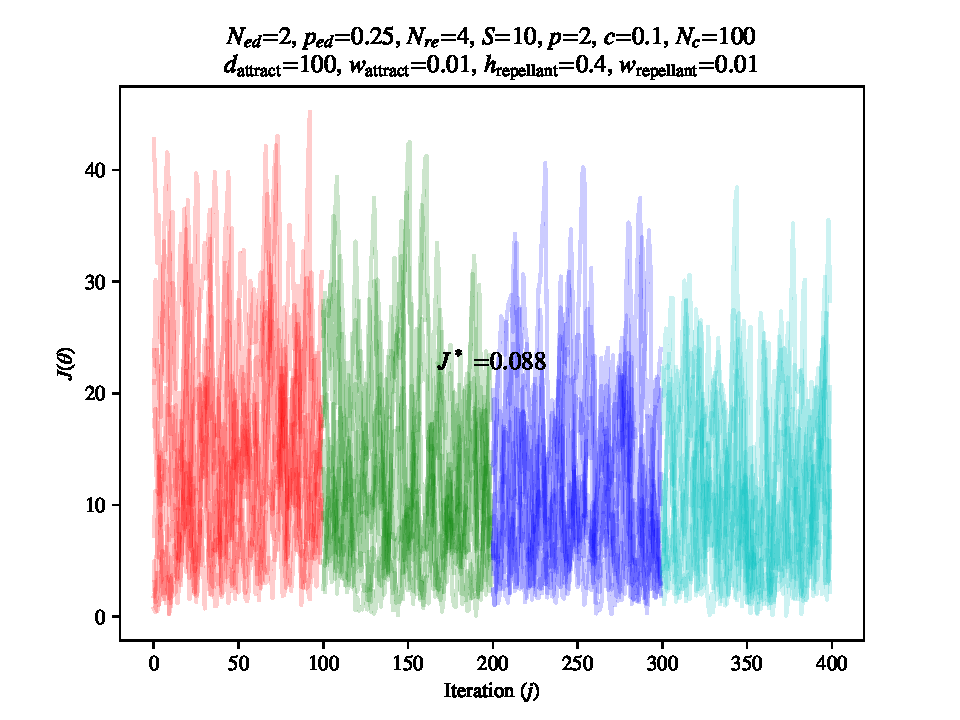
\includegraphics[scale=0.3]{assets/rastrigin_colony_ed_1_J}
    \end{center}
  \column{0.5\textwidth}
  \begin{center}
    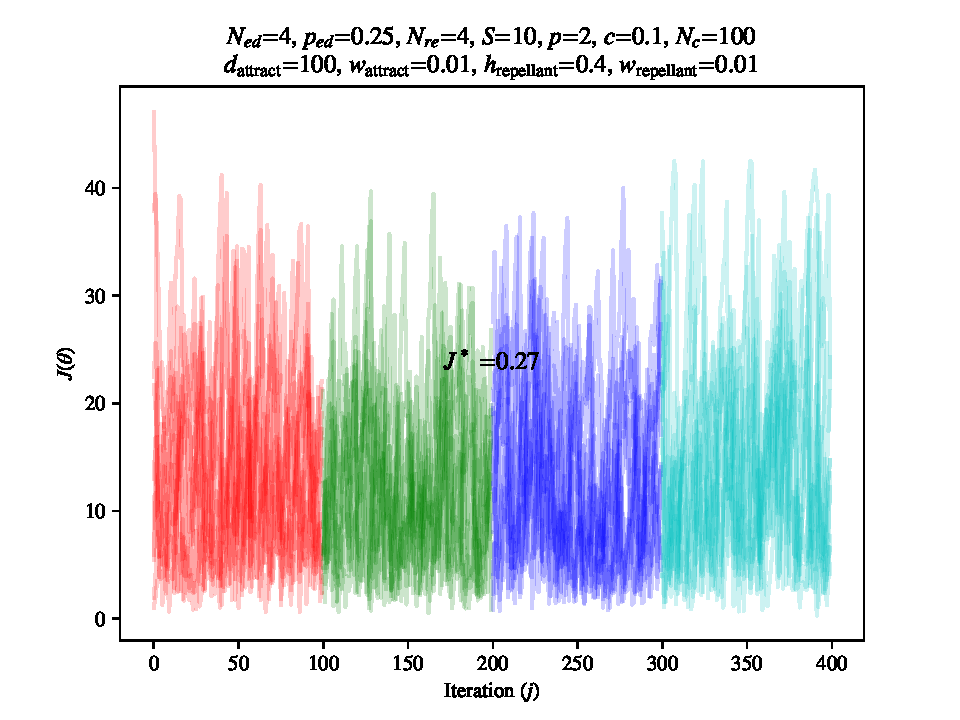
\includegraphics[scale=0.3]{assets/rastrigin_colony_ed_2_J}
    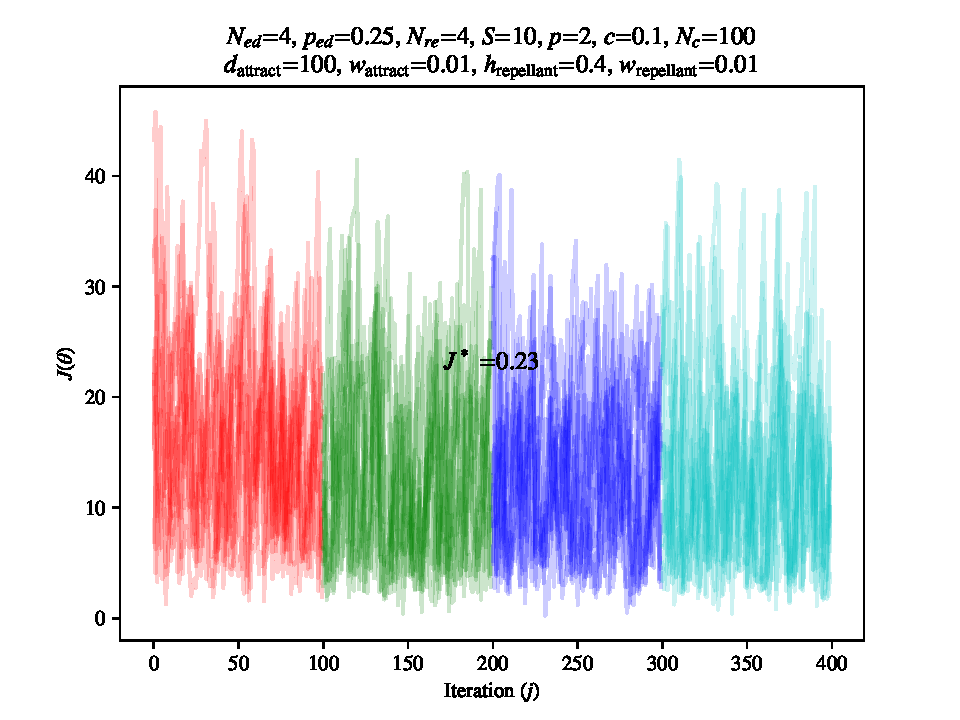
\includegraphics[scale=0.3]{assets/rastrigin_colony_ed_3_J}
  \end{center}
\end{columns}
\end{frame}

% I just want to discuss a few caveats of this exploration of this algorithm.
% First, I chose to use a highly nonconvex function to minimize. I chose to do this because I found that the function chosen by the author was quite simple with only a few local minima.
% It is definitely worth investigating this optimization algorithm with other test functions. I did try out some others, feel free to ask me about them during questions.
% I also set the random seed to 17 for all my experiments for reproducability purposes. If I had chosen a different seed, it's possible that I could get better or worse results
% I once tuned this algorithm's hyperparameters using this same algorithm with a fixed seed. It got awesome performance for that fixed seed, but the performance varied wildly by random seed.
\begin{frame}
\frametitle{Caveats}
\begin{itemize}
  \item<1-> This is only a single application:
  \begin{itemize}
    \item<1-> A single highly nonconvex function
    \item<1-> Should try out other loss functions and applications (see post-presentation slides)
  \end{itemize}
  \item<2-> Chose a single seed arbitrarily to run experiments:
  \begin{itemize}
    \item<2-> Results could vary if a different seed was chosen
  \end{itemize}
  \item<3-> Hyperparameters were chosen by trying a few random combinations
  \begin{itemize}
    \item<3-> Tried to avoid ``overfitting'' hyperparameters (abuse of terminology)
  \end{itemize}
\end{itemize}
\end{frame}

\section{Discussion}

% So here's a question. Is this a good optimization algorithm?
% Well, we don't know. The author doesn't compare to any existing optimization techniques.
% They spend some time comparing their algorithm to genetic algorithms since both are hill-climbing algorithms, but they insist that the algorithms are different because of what they are based on (rather than the actual algorithm itself).
% This is also quite similar to PSOs, using local/global information as well as a stochastic hill-climbing algorithm. Passino never mentions PSOs despite them being out for 7 years at the time of publication.
% I did compare this algorithm to PSOs though - ask me about it in the question period!
\begin{frame}
\frametitle{Is this a good optimization algorithm?}
\begin{itemize}
  \item<2-> We don't know. The author doesn't compare to any existing methods.
  \item<3-> The author draws a comparison to genetic algorithms (GAs) since both are hill-climbing algorithms, but asserts that they are really different algorithms \textbf{based on their biological inspiration}
  \item<4-> The method is also suspiciously similar to partical swarm optimization
  \begin{itemize}
    \item<5-> Combines local and global information with stochastic hill-climbing algorithm
    \item<5-> The author never mentions this despite the popularity of PSOs (this paper publish 7 years later)
    \item<6-> (Ask me about the comparison I did afterwards!)
  \end{itemize}
\end{itemize}
\end{frame}

% On the plus side, the algorithm is gradient-free. This means that we can optimize functions where we can't compute the gradient, such as tuning hyperparameters
% Versus random search and brute force, we don't need to know the range of the optimal value of theta.
\begin{frame}
\frametitle{Is this a good optimization algorithm?}
\begin{itemize}
  \item<1-> However, this algorithm is \textbf{gradient-free}
  \begin{itemize}
    \item<2-> We can minimize functions that we may not have access to the gradient for (or it may not exist)
    \item<2-> For example tuning hyperparameters
    \item<2-> Or for example fitting the parameters of a neural network to perform a task
  \end{itemize}
  \item<3-> It can also explore the search space beyond the initial distribution $d^0(\theta)$ in case we do not know where the optimal value $\theta^*$ lies
\end{itemize}
\end{frame}

% Here's another question. Is this a good model of E. coli?
% The truth is, we don't really know. The author doesn't validate his model using existing ecological data.
\begin{frame}
\frametitle{Is this a good model of \textit{E. coli}?}
\begin{itemize}
  \item<2-> We don't know. The author doesn't compare to any ecological data.
\end{itemize}
\end{frame}

% He does mention a few limitation of the model. I've chosen the most important ones, in my opinion, here.
% This is of course biologically-inspired and does not try to capture actual biological characteristics of E. coli except the essence of chemotaxis
% It ignores the actual medium itself, things like diffusion and consumption of nutrients
% Reproduction assumes a constant population size
% And the model for chemical signalling given by $J_cc$ is extremely oversimplified
\begin{frame}
\frametitle{Is this a good model of \textit{E. coli}?}
Some important limitations from the author:
\begin{itemize}
  \item<1> Ignore characteristics of actual biological processes in favor of simplicity and capturing the essence of chemotactic hill-climbing and swarming
  \item<2> Ignore characteristics of the chemical medium and  assume that consumption does not affect the nutrient surface
  \item<3> They assume a constant population size, even if there are many nutrients and generations
  \item<4> They assume that the cells respond to nutrients in the environment in the same way that they respond to ones released by other cells for the purpose of signaling the desire to swarm
\end{itemize}
\end{frame}

% Take a look at this screenshot directly from the paper. They have some giant text claiming they want to understand E. coli's foraging behaviour, and right next to it admit their real goals: a *simple* model of *certain* aspects of foraging behaviour.
% Also, after reading the paper, I still wasn't sure if the goal was to create a simulation of E. coli's foraging behaviour or to create another biologically-inspired metaheuristic.
\begin{frame}
\frametitle{Is this a good paper?}
\begin{center}
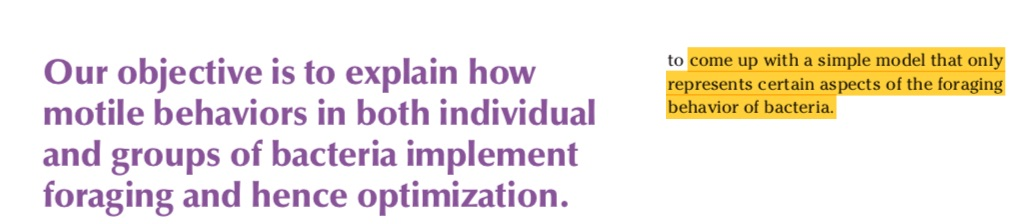
\includegraphics[scale=0.3]{assets/yikes}
\end{center}
\begin{itemize}
  \item<2-> It is not clear if the goal is create a simulation of \textit{E. coli} foraging behaviour or to create another biologically-inspired optimization algorithm
\end{itemize}
\end{frame}

% I'm now going to open the floor to discussion. Any questions or comments?
\begin{frame}
\frametitle{Discussion}
\end{frame}

\begin{frame}
\frametitle{Comparison to PSO}
\begin{itemize}
  \item Bacterial foraging method:
  \begin{itemize}
    \item   At least $N_{ed} \times N_{re} \times S \times N_c$ values of $\theta$ seen
  \end{itemize}
  \item PSO: $N \times \text{iter}$ values of $\theta$ seen
  \begin{itemize}
    \item PSO strongest with large $N$, so presume $\text{iter} \equiv N_c$
    \item Then $N = N_{ed} \times N_{re} \times S$
  \end{itemize}
\end{itemize}
\end{frame}

\begin{frame}
\frametitle{Comparison to PSO}
\begin{columns}[T]
  \column{0.5\textwidth}
    \begin{center}
      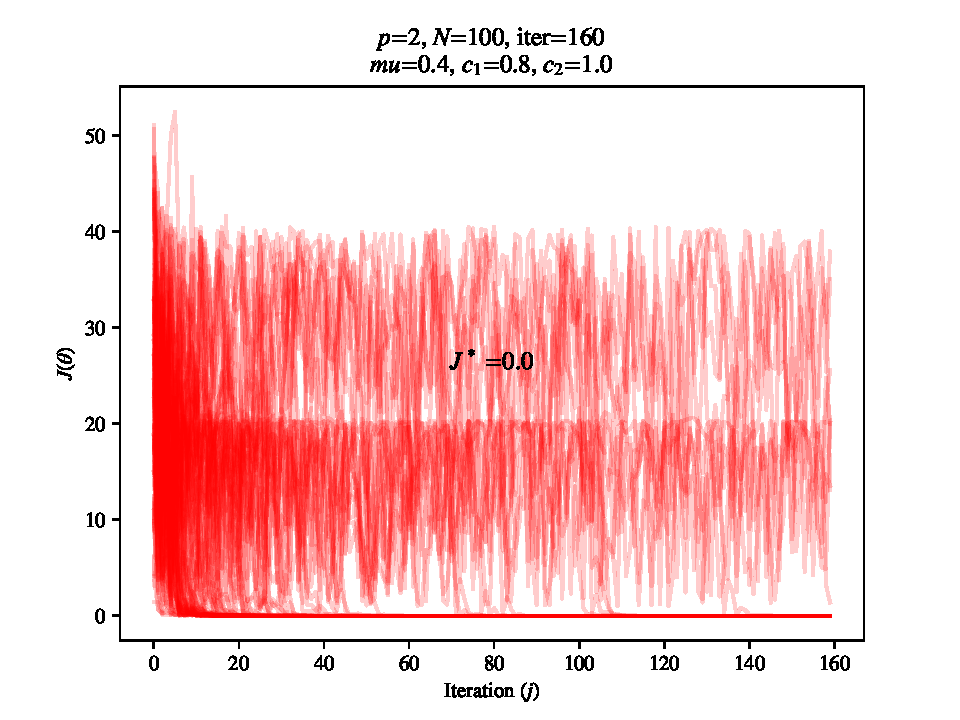
\includegraphics[scale=0.3]{assets/pso_J}
      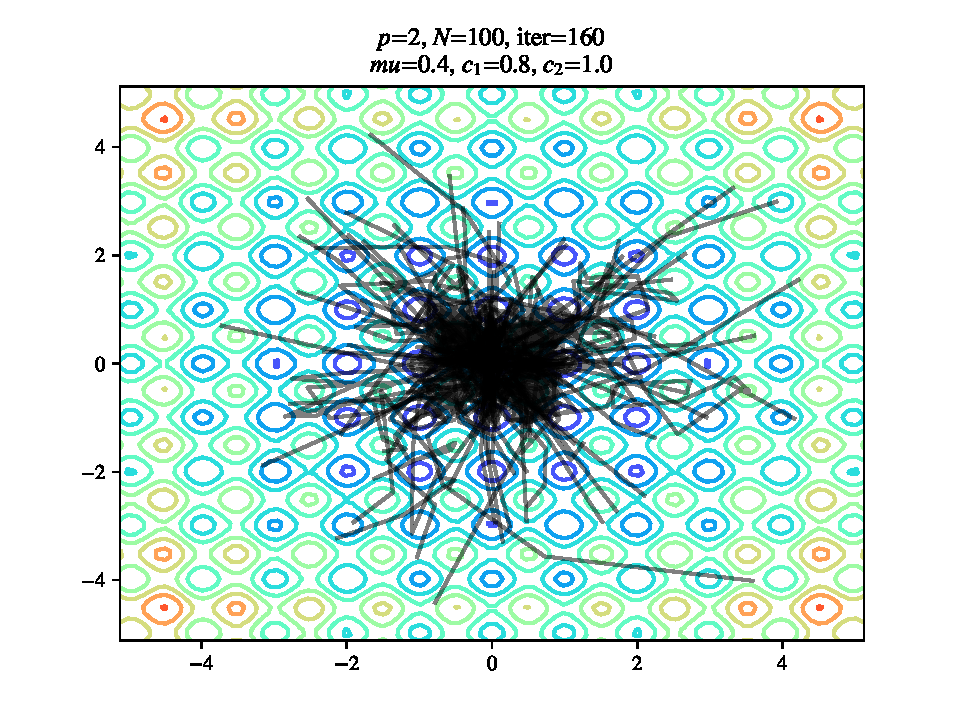
\includegraphics[scale=0.3]{assets/pso_theta}
    \end{center}
  \column{0.5\textwidth}
  \begin{center}
    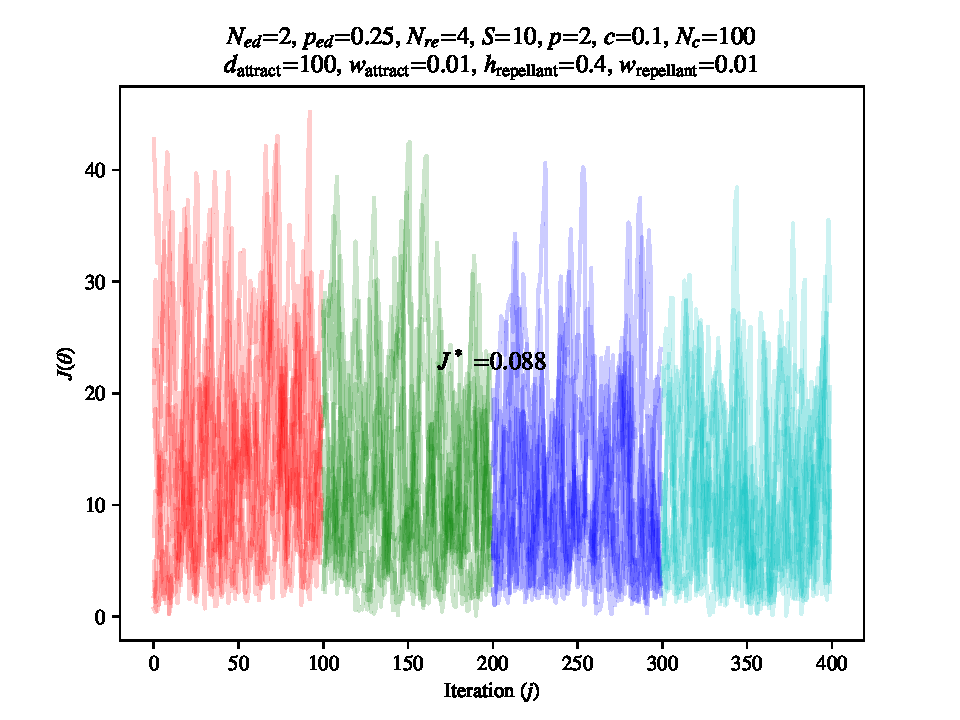
\includegraphics[scale=0.3]{assets/rastrigin_colony_ed_1_J}
    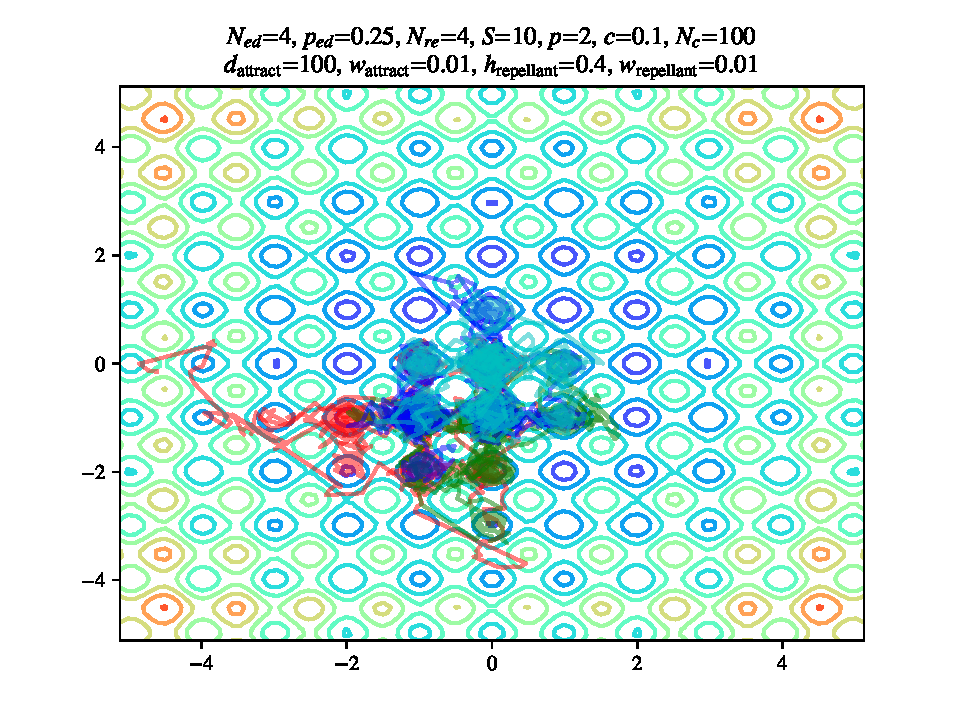
\includegraphics[scale=0.3]{assets/rastrigin_colony_ed_1_theta}
  \end{center}
\end{columns}
(Also, PSO is about 100x faster in my implementation.)
\end{frame}

\end{document}
